\documentclass[border=8pt]{standalone}
\usepackage[T1]{fontenc}
\usepackage{helvet}
\renewcommand{\familydefault}{\sfdefault}
\usepackage{tikz}
\usetikzlibrary{shapes.geometric, arrows.meta, positioning, calc}
\usepackage{xcolor}
\usepackage{booktabs}

\definecolor{dblue}{HTML}{1F4E79}
\definecolor{dgreen}{HTML}{2E7D32}
\definecolor{dpurple}{HTML}{755882}
\definecolor{lblue}{HTML}{E3F2FD}
\definecolor{lgreen}{HTML}{E8F5E9}
\definecolor{lpurple}{HTML}{F3E5F5}
\definecolor{lgray}{HTML}{F5F5F5}

\tikzset{
  phase/.style={draw=#1, fill=#1!8, rounded corners=8pt, line width=1.5pt,
    minimum width=16cm, inner sep=12pt},
  phasetitle/.style={font=\bfseries\Large, color=#1},
  arr/.style={-{Stealth[length=8pt]}, line width=2pt, color=gray!70},
  metricbox/.style={draw=gray!40, fill=lgray, rounded corners=4pt, line width=1pt,
    minimum width=16cm, inner sep=10pt},
}

\begin{document}
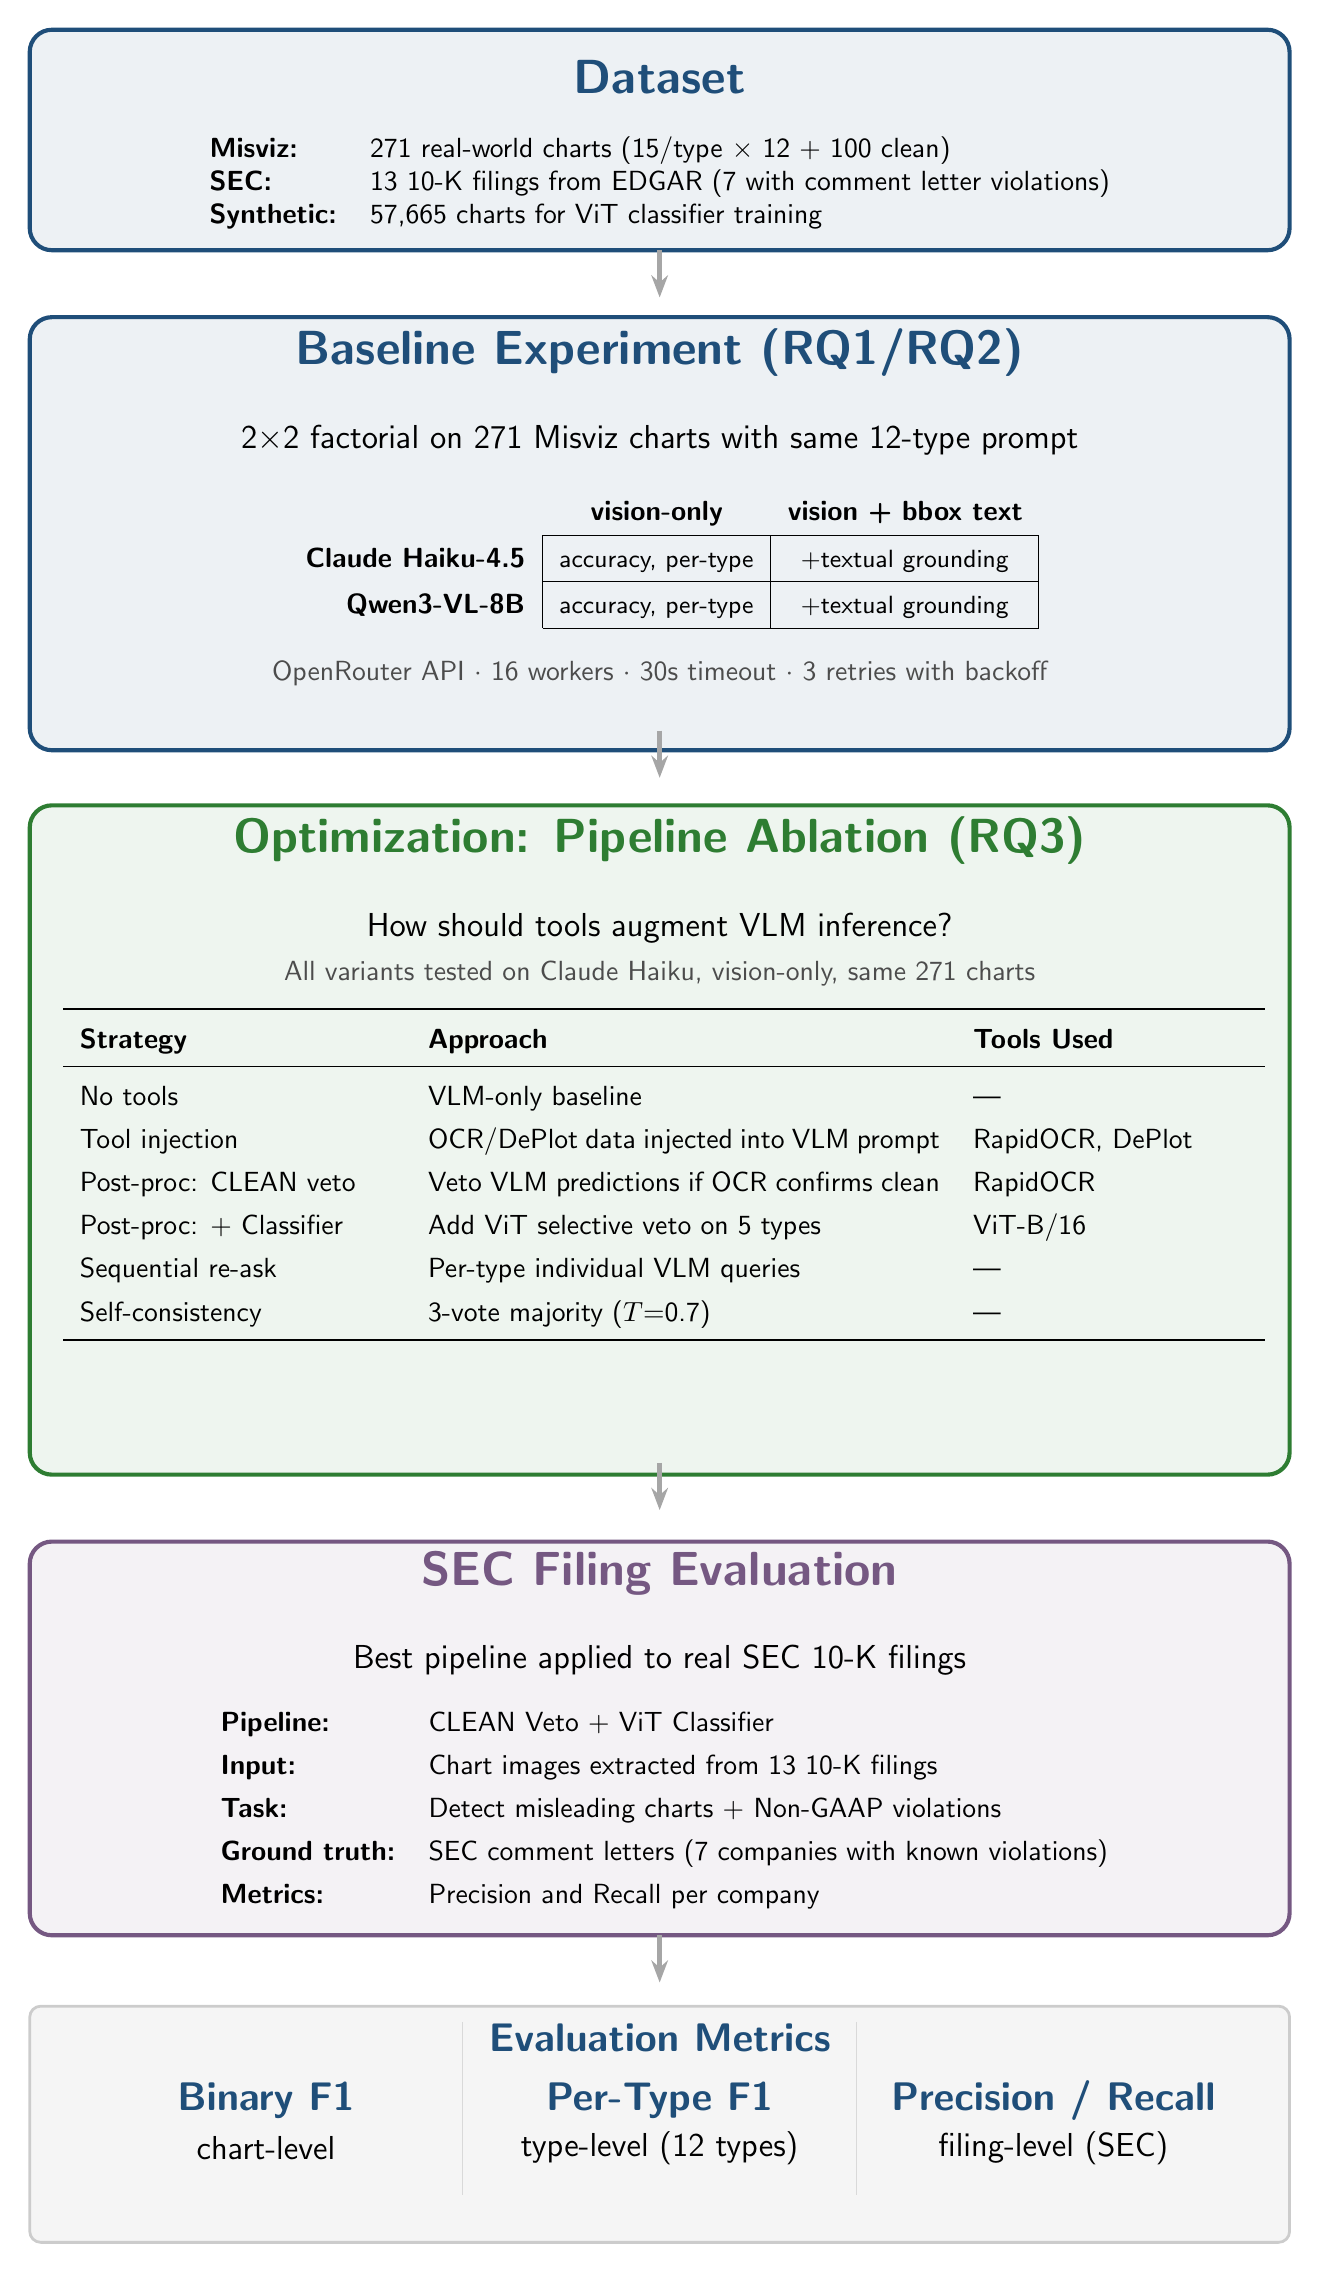
\begin{tikzpicture}[node distance=0.6cm]

% ══════════════════════════════════════════════════════
% DATASET
% ══════════════════════════════════════════════════════
\node[phase=dblue, minimum height=2.8cm] (dataset) at (0,0) {};
\node[phasetitle=dblue] at (0, 0.8) {\LARGE Dataset};
\node[anchor=north, font=\normalsize] at (0, 0.2) {%
  \begin{tabular}{ll}
    \textbf{Misviz:} & 271 real-world charts (15/type $\times$ 12 + 100 clean) \\
    \textbf{SEC:} & 13 10-K filings from EDGAR (7 with comment letter violations) \\
    \textbf{Synthetic:} & 57{,}665 charts for ViT classifier training \\
  \end{tabular}};

\draw[arr] (0,-1.4) -- (0,-2.0);

% ══════════════════════════════════════════════════════
% BASELINE (RQ1/RQ2)
% ══════════════════════════════════════════════════════
\node[phase=dblue, minimum height=5.5cm] at (0,-5.0) (baseline) {};
\node[phasetitle=dblue] at (0, -2.7) {\LARGE Baseline Experiment (RQ1/RQ2)};

\node[anchor=north, font=\large] at (0, -3.5) {%
  2$\times$2 factorial on 271 Misviz charts with same 12-type prompt};

\node[anchor=north, font=\normalsize] at (0, -4.3) {%
  \renewcommand{\arraystretch}{1.4}
  \begin{tabular}{r|c|c|}
    \multicolumn{1}{r}{} & \multicolumn{1}{c}{\textbf{vision-only}} & \multicolumn{1}{c}{\textbf{vision + bbox text}} \\
    \cline{2-3}
    \textbf{Claude Haiku-4.5} & \small accuracy, per-type & \small +textual grounding \\
    \cline{2-3}
    \textbf{Qwen3-VL-8B} & \small accuracy, per-type & \small +textual grounding \\
    \cline{2-3}
  \end{tabular}};

\node[anchor=north, font=\normalsize, color=black!70] at (0, -6.5) {%
  OpenRouter API $\cdot$ 16 workers $\cdot$ 30s timeout $\cdot$ 3 retries with backoff};

\draw[arr] (0,-7.5) -- (0,-8.1);

% ══════════════════════════════════════════════════════
% OPTIMIZATION (RQ3)
% ══════════════════════════════════════════════════════
\node[phase=dgreen, minimum height=8.5cm] at (0,-12.7) (optim) {};
\node[phasetitle=dgreen] at (0, -8.9) {\LARGE Optimization: Pipeline Ablation (RQ3)};

\node[anchor=north, font=\large] at (0, -9.7) {%
  How should tools augment VLM inference?};
\node[anchor=north, font=\normalsize, color=black!70] at (0, -10.3) {%
  All variants tested on Claude Haiku, vision-only, same 271 charts};

\node[anchor=north, font=\normalsize] at (0, -10.9) {%
  \renewcommand{\arraystretch}{1.3}
  \begin{tabular}{p{4cm}p{6.5cm}p{3.5cm}}
    \toprule
    \textbf{Strategy} & \textbf{Approach} & \textbf{Tools Used} \\
    \midrule
    No tools & VLM-only baseline & --- \\
    Tool injection & OCR/DePlot data injected into VLM prompt & RapidOCR, DePlot \\
    Post-proc: CLEAN veto & Veto VLM predictions if OCR confirms clean & RapidOCR \\
    Post-proc: + Classifier & Add ViT selective veto on 5 types & ViT-B/16 \\
    Sequential re-ask & Per-type individual VLM queries & --- \\
    Self-consistency & 3-vote majority ($T$=0.7) & --- \\
    \bottomrule
  \end{tabular}};

% removed sub-variant note

\draw[arr] (0,-16.8) -- (0,-17.4);

% ══════════════════════════════════════════════════════
% SEC EVALUATION
% ══════════════════════════════════════════════════════
\node[phase=dpurple, minimum height=5.0cm] at (0,-20.3) (sec) {};
\node[phasetitle=dpurple] at (0, -18.2) {\LARGE SEC Filing Evaluation};

\node[anchor=north, font=\large] at (0, -19.0) {%
  Best pipeline applied to real SEC 10-K filings};

\node[anchor=north, font=\normalsize] at (0, -19.7) {%
  \renewcommand{\arraystretch}{1.3}
  \begin{tabular}{ll}
    \textbf{Pipeline:} & CLEAN Veto + ViT Classifier \\
    \textbf{Input:} & Chart images extracted from 13 10-K filings \\
    \textbf{Task:} & Detect misleading charts + Non-GAAP violations \\
    \textbf{Ground truth:} & SEC comment letters (7 companies with known violations) \\
    \textbf{Metrics:} & Precision and Recall per company \\
  \end{tabular}};

\draw[arr] (0,-22.8) -- (0,-23.4);

% ══════════════════════════════════════════════════════
% METRICS
% ══════════════════════════════════════════════════════
\node[metricbox, minimum height=3.0cm] at (0,-25.2) (metrics) {};
\node[font=\bfseries\Large, color=dblue] at (0, -24.1) {Evaluation Metrics};

\node[font=\Large, color=dblue] at (-5, -24.9) {\textbf{Binary F1}};
\node[font=\large, color=black] at (-5, -25.5) {chart-level};

\node[font=\Large, color=dblue] at (0, -24.9) {\textbf{Per-Type F1}};
\node[font=\large, color=black] at (0, -25.5) {type-level (12 types)};

\node[font=\Large, color=dblue] at (5, -24.9) {\textbf{Precision / Recall}};
\node[font=\large, color=black] at (5, -25.5) {filing-level (SEC)};

\draw[gray!30] (-2.5,-23.9) -- (-2.5,-26.1);
\draw[gray!30] (2.5,-23.9) -- (2.5,-26.1);

\end{tikzpicture}
\end{document}
